\documentclass{beamer}
\usetheme{Boadilla}
\usepackage[utf8]{inputenc}
\usepackage{amsmath, amssymb}
\usepackage{tikz}
\usepackage{hyperref} %%%%TODO: anschauen wie man hyperrefs macht lol%%%%
\usetikzlibrary{external}
%\tikzexternalize[prefix=tikz/]


\begin{document}
    %%%illustr. of graph on page 1%%%%
    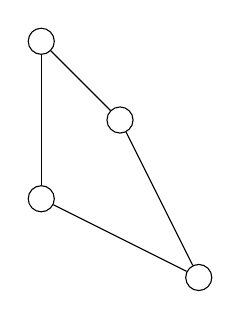
\begin{tikzpicture}[main/.style = {draw=black, circle}]
        \node[main] (1) at (0,0){};
        \node[main] (2) at (0,2){};
        \node[main] (3) at (1,1){};
        \node[main] (4) at (2,-1){};
        \draw[-] (1) -- (2);
        \draw[-] (1) -- (4);
        \draw[-] (2) -- (3);
        \draw[-] (3) -- (4);
    \end{tikzpicture}
    
    %%%%kein einfacher graph%%%%
%    \begin{tikzpicture}[main/.style = {draw=black, circle}]
%        \node[main] (1) at (5,-5){};
%        \draw[main] (1) arc (0.5:340:0.5);
%    \end{tikzpicture}
    
    %%%%not a simple graph%%%%
    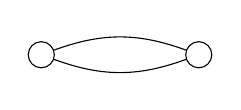
\begin{tikzpicture}[main/.style = {draw=black, circle}]
        \node[main] (1) at (8,-5){};
        \node[main] (2) at (10, -5){};
        \path[-] (1) edge[bend right=20] node[right] {}(2);
        \path[-] (1) edge[bend left=20] node [right] {} (2);
    \end{tikzpicture}
\end{document}